\documentclass[10pt,a4paper]{article}

\usepackage[margin=16mm,top=19mm,bottom=16mm,headheight=18pt,headsep=4mm,footskip=10mm]{geometry}
\usepackage{fontspec}
\usepackage{xcolor}
\usepackage{tikz}
\usepackage{booktabs}
\usepackage{tabularx}
\usepackage{array}
\usepackage{enumitem}
\usepackage{fancyhdr}
\usepackage{listings}
\usepackage[hidelinks]{hyperref}
\hypersetup{pdftitle={Shared Laboratory Equipment Booking System - IA3 Report},pdfauthor={Ansh, Arjun, Lakshit, Priyanshu}}
\usepackage{microtype}

% ---------- fonts ----------
\setmainfont{Avenir Next}
\newfontfamily\cond{Avenir Next Condensed}
\setmonofont{Menlo}
\newfontfamily\mono{Menlo}

% ---------- colours ----------
\definecolor{ink}{HTML}{16201E}
\definecolor{soft}{HTML}{4C5C58}
\definecolor{line}{HTML}{C2CDC8}
\definecolor{teal}{HTML}{0B6B62}
\definecolor{amber}{HTML}{A97517}
\definecolor{magenta}{HTML}{A31C4E}
\definecolor{codebg}{HTML}{F5F8F6}

\AtBeginDocument{\color{ink}\fontsize{9.0}{12.4}\selectfont}

\setlength{\parindent}{0pt}
\setlength{\parskip}{1.2mm}
\pagestyle{fancy}
\fancyhf{}
\renewcommand{\headrulewidth}{0.4pt}
\renewcommand{\footrulewidth}{0.4pt}
\renewcommand{\headrule}{\hbox to\headwidth{\color{line}\leaders\hrule height \headrulewidth\hfill}}
\renewcommand{\footrule}{\hbox to\headwidth{\color{line}\leaders\hrule height \footrulewidth\hfill}}
\fancyhead[L]{\mono\fontsize{7}{8}\selectfont\color{soft}\textbf{\color{teal}OOPS IN C++}\ /\ IA3 REPORT}
\fancyhead[R]{\mono\fontsize{7}{8}\selectfont\color{soft}\rightmark}
\fancyfoot[L]{\mono\fontsize{7}{8}\selectfont\color{soft}\leftmark}
\fancyfoot[R]{\mono\fontsize{7}{8}\selectfont\color{soft}\thepage\ /\ 2}

% ---------- helpers ----------
\newcommand{\code}[1]{\colorbox{codebg}{\texttt{\detokenize{#1}}}}
\newlength{\secpreskip}
\setlength{\secpreskip}{1.2mm}
\newcommand{\sechead}[1]{%
  \par\vspace{\secpreskip}%
  \noindent\begin{minipage}{\linewidth}%
    \setlength{\parskip}{0pt}%
    {\cond\bfseries\color{teal}\fontsize{13}{15}\selectfont #1\par}%
    \vspace{0.9mm}{\color{line}\hrule height 0.4pt}%
  \end{minipage}\par\vspace{1.0mm}%
}
\newcommand{\step}[3]{%
  \begin{minipage}[t]{0.232\linewidth}
    \setlength{\parskip}{0pt}%
    {\color{teal}\rule{\linewidth}{1.1pt}}\par\vspace{1.2mm}
    {\mono\fontsize{6.3}{7.5}\selectfont\color{amber}STEP #1}\par\vspace{0.4mm}
    {\bfseries\fontsize{9.4}{11}\selectfont #2}\par\vspace{0.3mm}
    {\fontsize{7.5}{9.4}\selectfont\color{soft} #3}
  \end{minipage}%
}

\lstset{
  basicstyle=\mono\fontsize{7.2}{8.7}\selectfont,
  backgroundcolor=\color{codebg},
  frame=none,
  xleftmargin=4mm,
  xrightmargin=0mm,
  aboveskip=1mm,
  belowskip=1mm,
  escapeinside={(*}{*},
  columns=fullflexible,
  keepspaces=true,
  showstringspaces=false,
}

% diagram styles
\tikzset{
  clsbox/.style={draw=teal, fill=white, line width=0.5pt},
  clshead/.style={anchor=west, text=white, inner sep=0pt,
    font=\cond\bfseries\fontsize{8}{9}\selectfont},
  clsbody/.style={anchor=north west, align=left, text=ink, inner sep=0pt,
    font=\mono\fontsize{5.6}{7.1}\selectfont},
  childbox/.style={draw=teal, fill=codebg, line width=0.4pt},
  childhead/.style={anchor=north west, inner sep=0pt,
    font=\cond\bfseries\fontsize{6.6}{7.4}\selectfont, text=ink},
  childbody/.style={anchor=north west, inner sep=0pt,
    font=\mono\fontsize{5.15}{6.4}\selectfont, text=soft},
}

\begin{document}

\markboth{Shared Laboratory Equipment Booking System}{28 October 2026}

% ================= PAGE 1 =================
{\cond\bfseries\fontsize{25}{26}\selectfont
Shared Laboratory Equipment Booking System\par}
\vspace{1.2mm}
{\fontsize{10.4}{13}\selectfont\color{soft}
A C++ console application that records who has which lab instrument, when it is due, and what a late return costs.\par}
\vspace{3mm}
{\mono\fontsize{7.4}{9}\selectfont
\textbf{Team}\ \ Ansh\quad Arjun\quad Lakshit\quad Priyanshu\hspace{8mm}%
\textbf{Repo}\ \ \href{https://github.com/vee1e/lab-booking-system}{\textcolor{teal}{github.com/vee1e/lab-booking-system}}\par}

\sechead{1. Problem}
The lab shares its microscopes, centrifuges and spectrometers between students and staff. Nothing records who holds what, so two people can claim the same instrument, and a late return leaves no trace. We built a menu-driven program that keeps that record in memory: it tracks each item's state, each user's quota and loan period, and every borrow and return.

\sechead{2. How it works}
\noindent
\step{01}{Sign in}{Pick a user. The role sets the item limit, loan length and fine rate.}\hfill
\step{02}{See the shelf}{Menu 2 lists every instrument as FREE or TAKEN, with its type and spec.}\hfill
\step{03}{Borrow}{Checks availability and quota, then writes a booking with a due day.}\hfill
\step{04}{Return}{Closes the booking and charges the fine if the return is past due.}

\vspace{1.2mm}
{\fontsize{7.3}{9}\selectfont\color{soft}Other menu actions: booking log, search by word or id, user list, admin add, admin remove, advance day, exit.\par}

\sechead{3. Class design}
\begin{center}
\resizebox{\linewidth}{!}{%
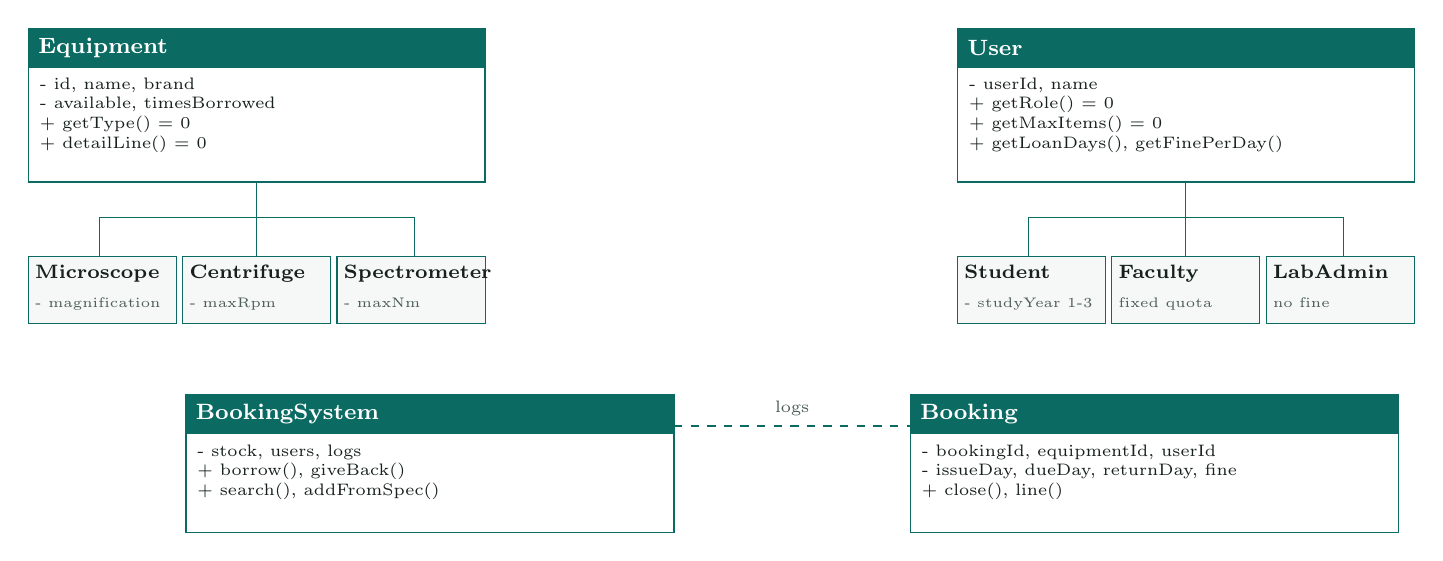
\begin{tikzpicture}[x=1cm,y=1cm]
  % ---- Equipment ----
  \draw[clsbox] (0,7.7) rectangle (5.8,5.75);
  \fill[teal] (0,7.7) rectangle (5.8,7.2);
  \node[clshead] at (0.12,7.45) {Equipment};
  \node[clsbody] at (0.14,7.08) {- id, name, brand \\ - available, timesBorrowed \\ + getType() = 0 \\ + detailLine() = 0};

  % ---- User ----
  \draw[clsbox] (11.8,7.7) rectangle (17.6,5.75);
  \fill[teal] (11.8,7.7) rectangle (17.6,7.2);
  \node[clshead] at (11.92,7.45) {User};
  \node[clsbody] at (11.94,7.08) {- userId, name \\ + getRole() = 0 \\ + getMaxItems() = 0 \\ + getLoanDays(), getFinePerDay()};

  % ---- inheritance lines ----
  \draw[teal,line width=0.4pt] (2.9,5.75) -- (2.9,5.3);
  \draw[teal,line width=0.4pt] (0.9,5.3) -- (4.9,5.3);
  \draw[teal,line width=0.4pt] (0.9,5.3) -- (0.9,4.8);
  \draw[teal,line width=0.4pt] (2.9,5.3) -- (2.9,4.8);
  \draw[teal,line width=0.4pt] (4.9,5.3) -- (4.9,4.8);

  \draw[teal,line width=0.4pt] (14.7,5.75) -- (14.7,5.3);
  \draw[teal,line width=0.4pt] (12.7,5.3) -- (16.7,5.3);
  \draw[teal,line width=0.4pt] (12.7,5.3) -- (12.7,4.8);
  \draw[teal,line width=0.4pt] (14.7,5.3) -- (14.7,4.8);
  \draw[teal,line width=0.4pt] (16.7,5.3) -- (16.7,4.8);

  % ---- equipment children ----
  \draw[childbox] (0,4.8) rectangle (1.88,3.95);
  \node[childhead] at (0.08,4.7) {Microscope};
  \node[childbody] at (0.08,4.28) {- magnification};

  \draw[childbox] (1.96,4.8) rectangle (3.84,3.95);
  \node[childhead] at (2.04,4.7) {Centrifuge};
  \node[childbody] at (2.04,4.28) {- maxRpm};

  \draw[childbox] (3.92,4.8) rectangle (5.8,3.95);
  \node[childhead] at (4.0,4.7) {Spectrometer};
  \node[childbody] at (4.0,4.28) {- maxNm};

  % ---- user children ----
  \draw[childbox] (11.8,4.8) rectangle (13.68,3.95);
  \node[childhead] at (11.88,4.7) {Student};
  \node[childbody] at (11.88,4.28) {- studyYear 1-3};

  \draw[childbox] (13.76,4.8) rectangle (15.64,3.95);
  \node[childhead] at (13.84,4.7) {Faculty};
  \node[childbody] at (13.84,4.28) {fixed quota};

  \draw[childbox] (15.72,4.8) rectangle (17.6,3.95);
  \node[childhead] at (15.8,4.7) {LabAdmin};
  \node[childbody] at (15.8,4.28) {no fine};

  % ---- BookingSystem ----
  \draw[clsbox] (2.0,3.05) rectangle (8.2,1.3);
  \fill[teal] (2.0,3.05) rectangle (8.2,2.55);
  \node[clshead] at (2.12,2.8) {BookingSystem};
  \node[clsbody] at (2.14,2.42) {- stock, users, logs \\ + borrow(), giveBack() \\ + search(), addFromSpec()};

  % ---- Booking ----
  \draw[clsbox] (11.2,3.05) rectangle (17.4,1.3);
  \fill[teal] (11.2,3.05) rectangle (17.4,2.55);
  \node[clshead] at (11.32,2.8) {Booking};
  \node[clsbody] at (11.34,2.42) {- bookingId, equipmentId, userId \\ - issueDay, dueDay, returnDay, fine \\ + close(), line()};

  % ---- link ----
  \draw[teal,line width=0.4pt,dashed] (8.2,2.65) -- (11.2,2.65);
  \node[font=\mono\fontsize{5.8}{7}\selectfont,text=soft,above] at (9.7,2.65) {logs};
\end{tikzpicture}}
\end{center}
\vspace{-1mm}
{\fontsize{7.2}{9}\selectfont\color{soft}Solid lines show inheritance. The dashed line shows that BookingSystem stores Booking records by value, while items and users are owned through pointers.\par}

\sechead{4. Role rules}
\renewcommand{\arraystretch}{1.15}
\begin{tabularx}{\linewidth}{@{}lrrrl@{}}
\toprule
{\mono\fontsize{6.3}{7.5}\selectfont\color{soft}ROLE} &
{\mono\fontsize{6.3}{7.5}\selectfont\color{soft}MAX ITEMS} &
{\mono\fontsize{6.3}{7.5}\selectfont\color{soft}LOAN} &
{\mono\fontsize{6.3}{7.5}\selectfont\color{soft}FINE PER LATE DAY} &
{\mono\fontsize{6.3}{7.5}\selectfont\color{soft}SOURCE} \\
\midrule
Student, year 1 & 2 & 7 days & 10 & \code{User.h} \\
Student, year 2 & 3 & 7 days & 10 & \code{User.h} \\
Student, year 3 & 4 & 7 days & 10 & \code{User.h} \\
Faculty & 5 & 14 days & 5 & \code{User.h} \\
Lab Admin & 10 & 30 days & 0 & \code{User.h} \\
\bottomrule
\end{tabularx}
\vspace{0.8mm}

{\fontsize{7.2}{9}\selectfont\color{soft}The fine rate and loan length come from the signed-in user's role. Booking due day = issue day + loan days.\par}

\sechead{5. Three states on screen}
\noindent
\begin{minipage}[t]{0.315\linewidth}
  \setlength{\parskip}{0pt}%
  {\color{teal}\rule{\linewidth}{1.2pt}}\par\vspace{0.6mm}
  {\mono\fontsize{7}{8}\selectfont\color{teal}FREE}\par\vspace{0.6mm}
  {\bfseries\fontsize{9}{10.5}\selectfont On the shelf}\par\vspace{0.5mm}
  {\fontsize{7.4}{9}\selectfont\color{soft}The item is free. Anyone under their item limit can borrow it.}
\end{minipage}\hfill
\begin{minipage}[t]{0.315\linewidth}
  \setlength{\parskip}{0pt}%
  {\color{amber}\rule{\linewidth}{1.2pt}}\par\vspace{0.8mm}
  {\mono\fontsize{7}{8}\selectfont\color{amber}TAKEN}\par\vspace{0.6mm}
  {\bfseries\fontsize{9}{10.5}\selectfont Already out}\par\vspace{0.5mm}
  {\fontsize{7.4}{9}\selectfont\color{soft}A second borrow is refused, and the message names the holder.}
\end{minipage}\hfill
\begin{minipage}[t]{0.315\linewidth}
  \setlength{\parskip}{0pt}%
  {\color{magenta}\rule{\linewidth}{1.2pt}}\par\vspace{0.8mm}
  {\mono\fontsize{7}{8}\selectfont\color{magenta}LATE}\par\vspace{0.6mm}
  {\bfseries\fontsize{9}{10.5}\selectfont Past the due day}\par\vspace{0.5mm}
  {\fontsize{7.4}{9}\selectfont\color{soft}The return is accepted, and the days late and the amount owed appear.}
\end{minipage}

\newpage
% ================= PAGE 2 =================
\setlength{\secpreskip}{2.6mm}
\markboth{Ansh\quad Arjun\quad Lakshit\quad Priyanshu}{Design notes and results}

\sechead{6. OOP features in the code}
\renewcommand{\arraystretch}{1.12}
\setlength{\tabcolsep}{2mm}
\begin{tabularx}{\linewidth}{@{}p{3.1cm}X@{}}
\toprule
{\mono\fontsize{6.3}{7.5}\selectfont\color{soft}FEATURE} &
{\mono\fontsize{6.3}{7.5}\selectfont\color{soft}WHERE IT IS USED} \\
\midrule
\textbf{Encapsulation} & All state is private. \code{available} changes only through \code{markBorrowed()} and \code{markReturned()}; a booking closes only through \code{close()}. Outside code reads state through const getters. \\
\addlinespace[0.8mm]
\textbf{Inheritance} & \code{Equipment} has three children (\code{Microscope}, \code{Centrifuge}, \code{Spectrometer}); \code{User} has three (\code{Student}, \code{Faculty}, \code{LabAdmin}). Each child adds one field or one rule set. \\
\addlinespace[0.8mm]
\textbf{Abstraction} & \code{getType()} and \code{detailLine()} are pure virtual, and so are the four \code{User} rule methods. No \code{Equipment} or \code{User} object can exist on its own. \\
\addlinespace[0.8mm]
\textbf{Polymorphism} & The system holds \code{vector<Equipment*>} and \code{vector<User*>}. List, search and quota checks call the child version through the base pointer, with no type checks. \\
\addlinespace[0.8mm]
\textbf{Overloading} & Two constructors for each instrument type and for \code{Student} (full spec or default), and two \code{search} functions, one taking a \code{string} and one taking an \code{int}. \\
\addlinespace[0.8mm]
\textbf{Composition} & \code{BookingSystem} owns the item and user lists and deletes them in its destructor. \code{Booking} stores ids instead of pointers, so an old record cannot dangle after an item is removed. \\
\bottomrule
\end{tabularx}
\vspace{0.8mm}

{\fontsize{7.2}{9}\selectfont\color{soft}Also used: static id counters shared by each class, default arguments, friend \code{operator<<}, and two plain structs, \code{Result} (ok flag plus message) and \code{GearSpec} (one creation pack).\par}

\vspace*{1mm}
\sechead{7. Borrow rules and refusals}
\begin{minipage}[t]{0.485\linewidth}
Borrowing is refused when the item is already out (the message names the holder) or the user is at their role's item limit (the message gives the count and the limit). Removing an item is refused while it is still out.

Borrow and return also require a signed-in user. Borrow, return, add and remove each return a \code{Result} with a full sentence, so the screen never shows a bare error code. Non-numeric menu input is rejected and re-asked instead of leaving \code{cin} in a failed state.
\end{minipage}\hfill
\begin{minipage}[t]{0.485\linewidth}
Rules live in one place, \code{BookingSystem::borrow} and \code{giveBack}. The menu only reads input and prints the message, so a rule change does not touch the interface.

The log keeps closed records too, so the history stays readable after an item is back on the shelf.

\vspace{0.5mm}
\colorbox{codebg}{\parbox{0.94\linewidth}{\mono\fontsize{7.2}{9}\selectfont B5001 gear=101 user=1 issue=1 due=8 back=9 fine=10}}
\end{minipage}

\vspace*{1mm}
\sechead{8. Sample run}
\begin{lstlisting}
(*\textcolor{soft}{\# borrow the microscope, request it again, then return on day 9}*)
> 3   101
(*\textcolor{teal}{OK: Priyanshu took 'Olympus CX23' [Microscope] on day 1. Due day 8 (loan 7 days for Student).}*)
> 3   101
(*\textcolor{magenta}{FAIL: 'Olympus CX23' is TAKEN by user 1. Pick another id from menu 2.}*)
> 4   101
(*\textcolor{teal}{OK but LATE: day 9 is past due 8. Fine=10 (1 day x 10/day).}*)
\end{lstlisting}
\vspace{0.5mm}
{\fontsize{7.2}{9}\selectfont\color{soft}Output from the built binary, trimmed to the lines that matter. The full run also covers quota refusal, a second user, search by word and id, and admin add and remove.\par}

\sechead{9. Limits and next steps}
\begin{minipage}[t]{0.485\linewidth}
{\mono\fontsize{6.3}{7.5}\selectfont\color{soft}CURRENT LIMITS}\par\vspace{0.8mm}
{\fontsize{8.2}{10.2}\selectfont
\begin{itemize}[leftmargin=4mm,itemsep=0.35mm,topsep=0pt,parsep=0pt]
  \item Nothing is saved. Closing the program resets the register.
  \item Dates are a manual day counter, not real dates.
  \item One terminal session at a time, with no concurrent users.
  \item Menus 9 and 10 do not check for the Lab Admin role.
  \item Checks are manual. There are no automated tests.
\end{itemize}}
\end{minipage}\hfill
\begin{minipage}[t]{0.485\linewidth}
{\mono\fontsize{6.3}{7.5}\selectfont\color{soft}NEXT STEPS}\par\vspace{0.8mm}
{\fontsize{8.2}{10.2}\selectfont
\begin{itemize}[leftmargin=4mm,itemsep=0.35mm,topsep=0pt,parsep=0pt,label={\color{teal}\textbullet}]
  \item Save and load the register from a file.
  \item Use real dates for issue and due days.
  \item Restrict add and remove to the admin role.
  \item Add unit tests for the quota, availability and fine rules.
\end{itemize}}
\end{minipage}

\sechead{10. Build}
Build with \code{g++ -std=c++17 -Wall main.cpp -o labbook}, then run \code{./labbook}. C++17 and the standard library only, with no database and no third-party dependency. The same menu and rules are also ported to the browser at \href{https://lab-booking-system-mu.vercel.app/\#shell}{lab-booking-system-mu.vercel.app/\#shell}.

The build is clean under \code{-Wall}. A scripted run covered login, a borrow, duplicate and quota refusals, a late fine, both searches, and admin add and remove.

\end{document}
